\documentclass{beamer}
\usepackage{relsize}
\usepackage{color}

\usepackage{listings}
\usetheme{CambridgeUS}
%\usepackage{beamerthemesplit} % new
\usepackage{enumitem}
\usepackage{amsmath}                    % See geometry.pdf to learn the layout options.
\usepackage{amsthm}                   % See geometry.pdf to learn the layout options. There
\usepackage{amssymb}                    % See geometry.pdf to learn the layout options.
\usepackage[utf8]{inputenc}
\usepackage{graphicx}
\usepackage[english,bulgarian]{babel}

\usepackage{caption}
\usepackage{tikz}

\usetheme{CambridgeUS}
\usecolortheme{crane}

\lstset{language=C++,
                basicstyle=\ttfamily,
                keywordstyle=\color{blue}\ttfamily,
                stringstyle=\color{red}\ttfamily,
                commentstyle=\color{green}\ttfamily,
                morecomment=[l][\color{magenta}]{\#}
}

\newtheorem{mydef}{Дефиниция}[section]
\newtheorem{lem}{Лема}[section]
\newtheorem{thm}{Твърдение}[section]

\DeclareMathOperator{\restrict}{\upharpoonright}

\setitemize{label=\usebeamerfont*{itemize item}%
  \usebeamercolor[fg]{itemize item}
  \usebeamertemplate{itemize item}}

\setbeamercovered{transparent}

\captionsetup{font=tiny} 

\begin{document}
\title[Вход / изход]{Вход / изход}
\frame{\titlepage}

\section{Вход / изход}
\subsection{}

\begin{frame}[fragile]
  \frametitle{Чисто функционално програмиране}
  \begin{tikzpicture}[remember picture,overlay]
    \node[xshift=0,yshift=-14mm,anchor=north] at (current page.north){%
    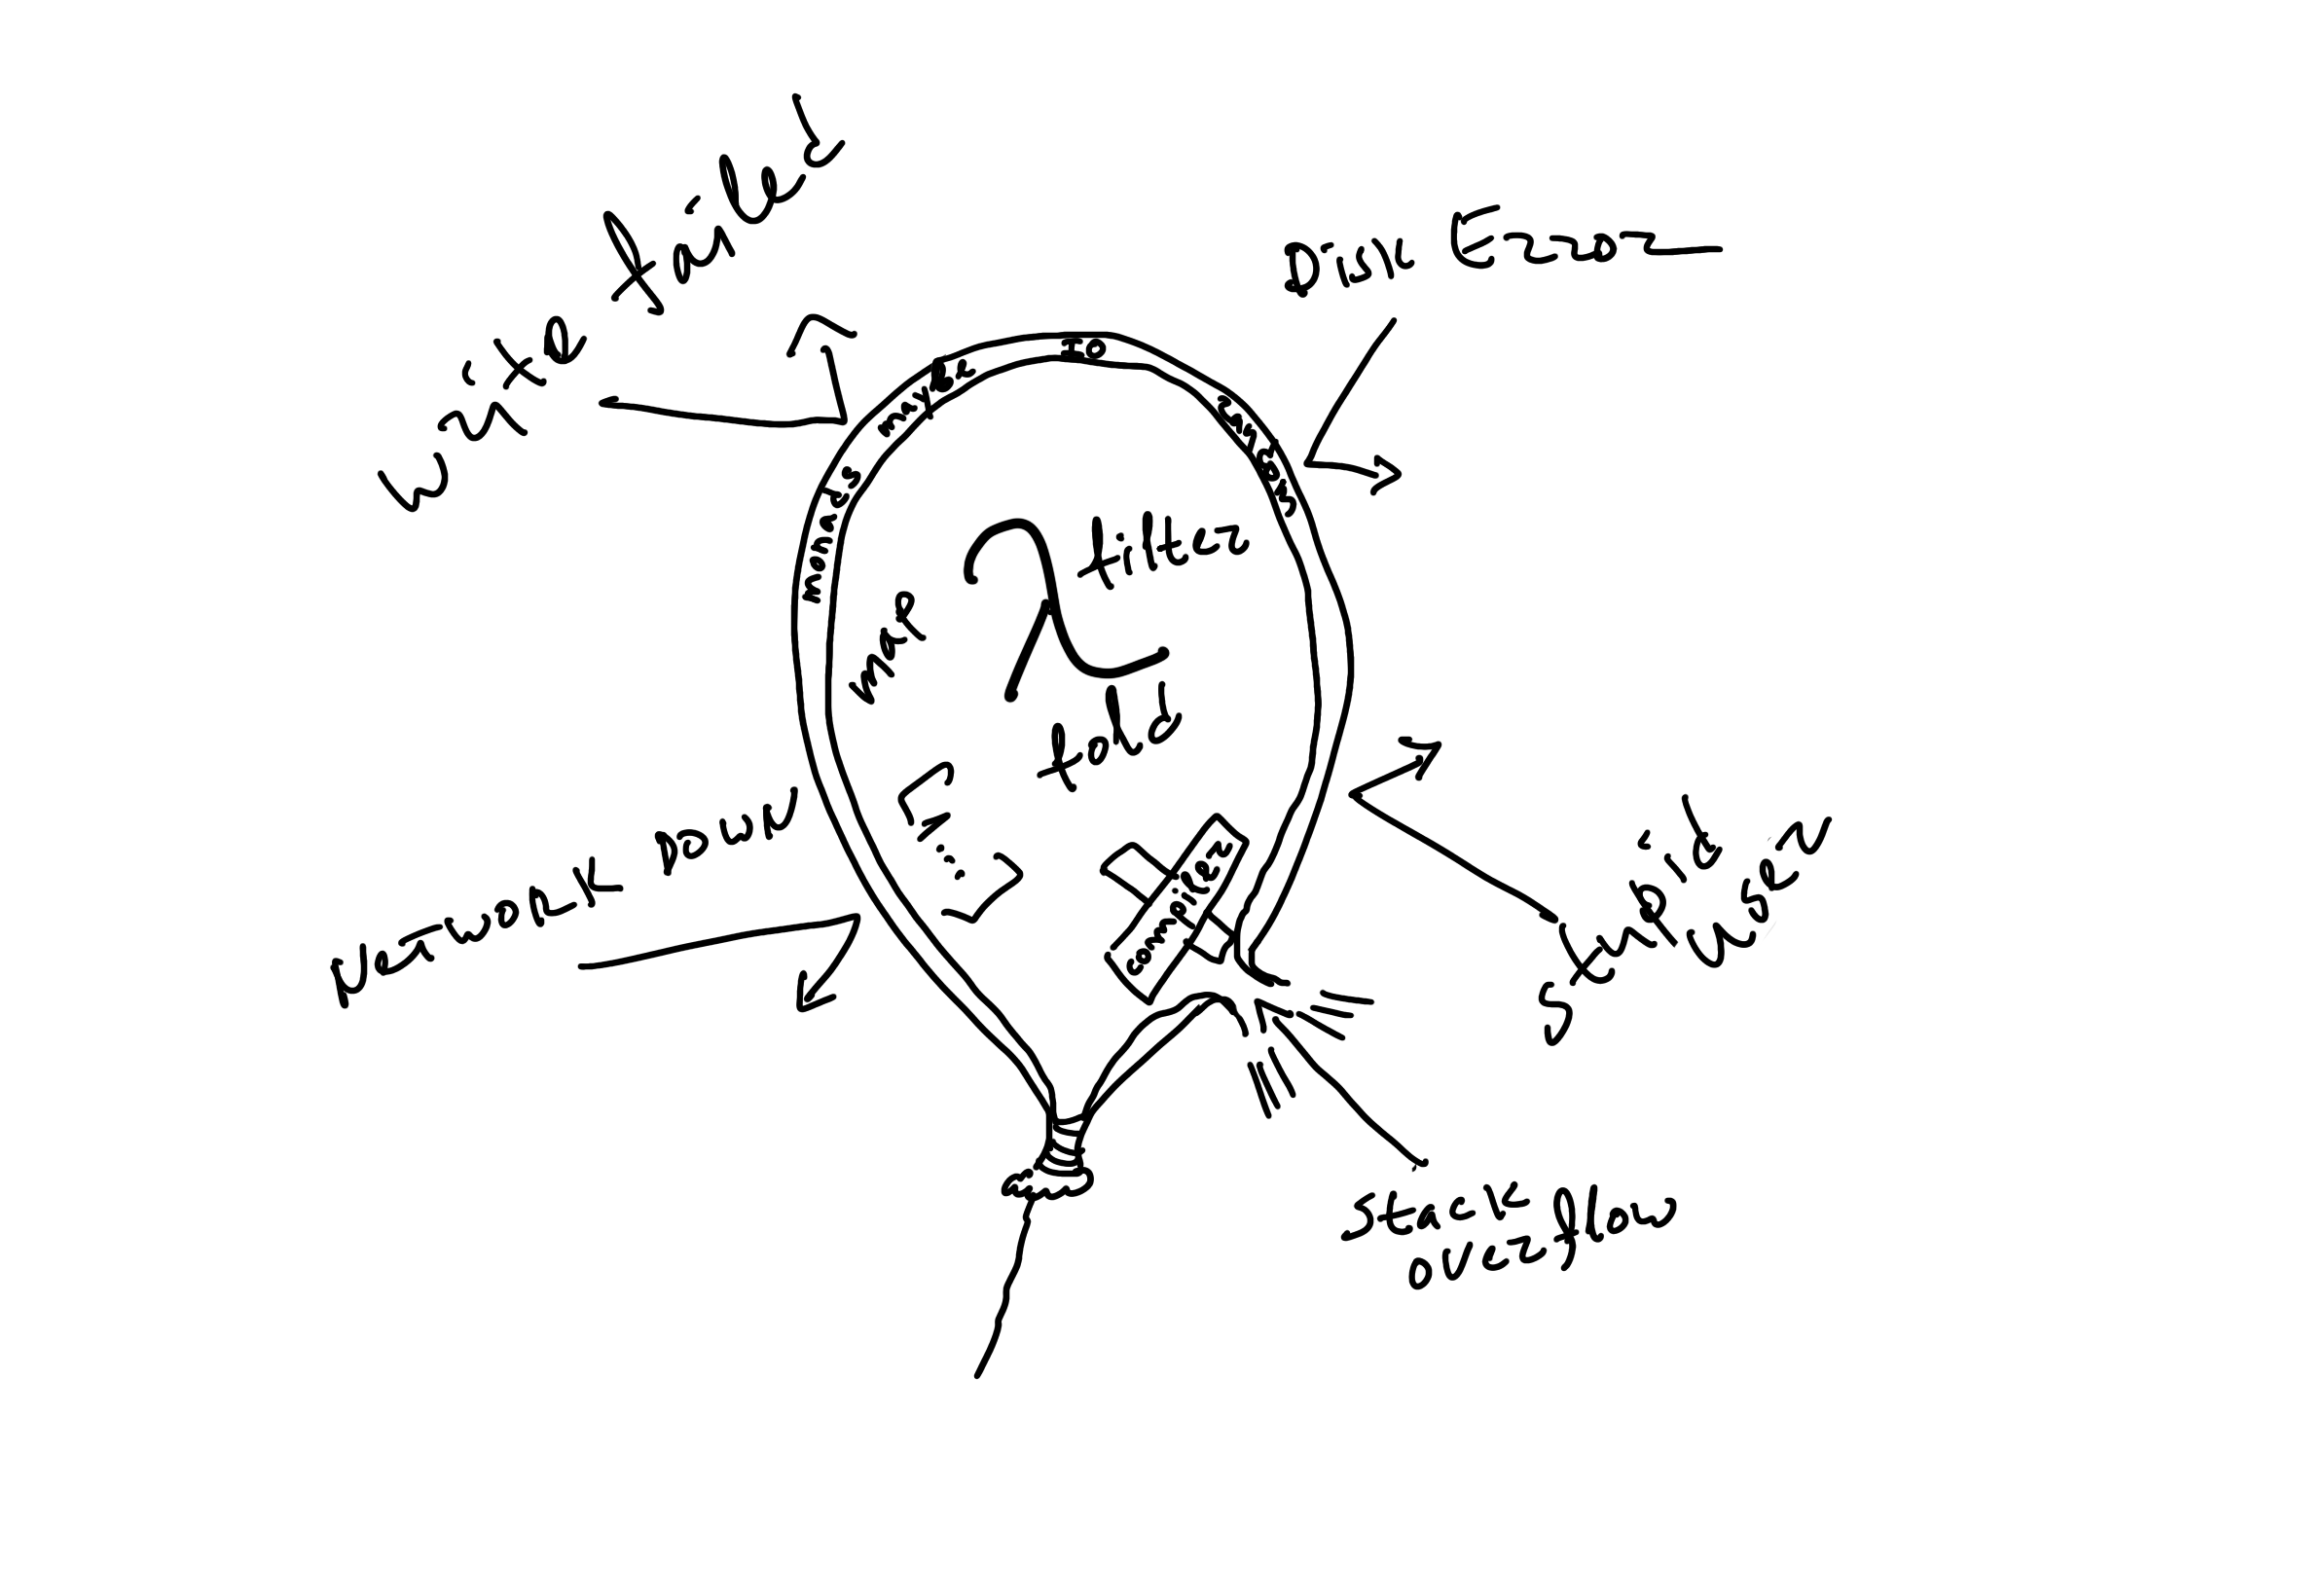
\includegraphics[width=120mm]{images/pure_functional}};
  \end{tikzpicture}
\end{frame}



\begin{frame}[fragile]
  \frametitle{Да си припомним Maybe монада}

\begin{tikzpicture}[remember picture,overlay]
  \node[xshift=0mm,yshift=-10mm,anchor=north east] at (current page.north east){%
  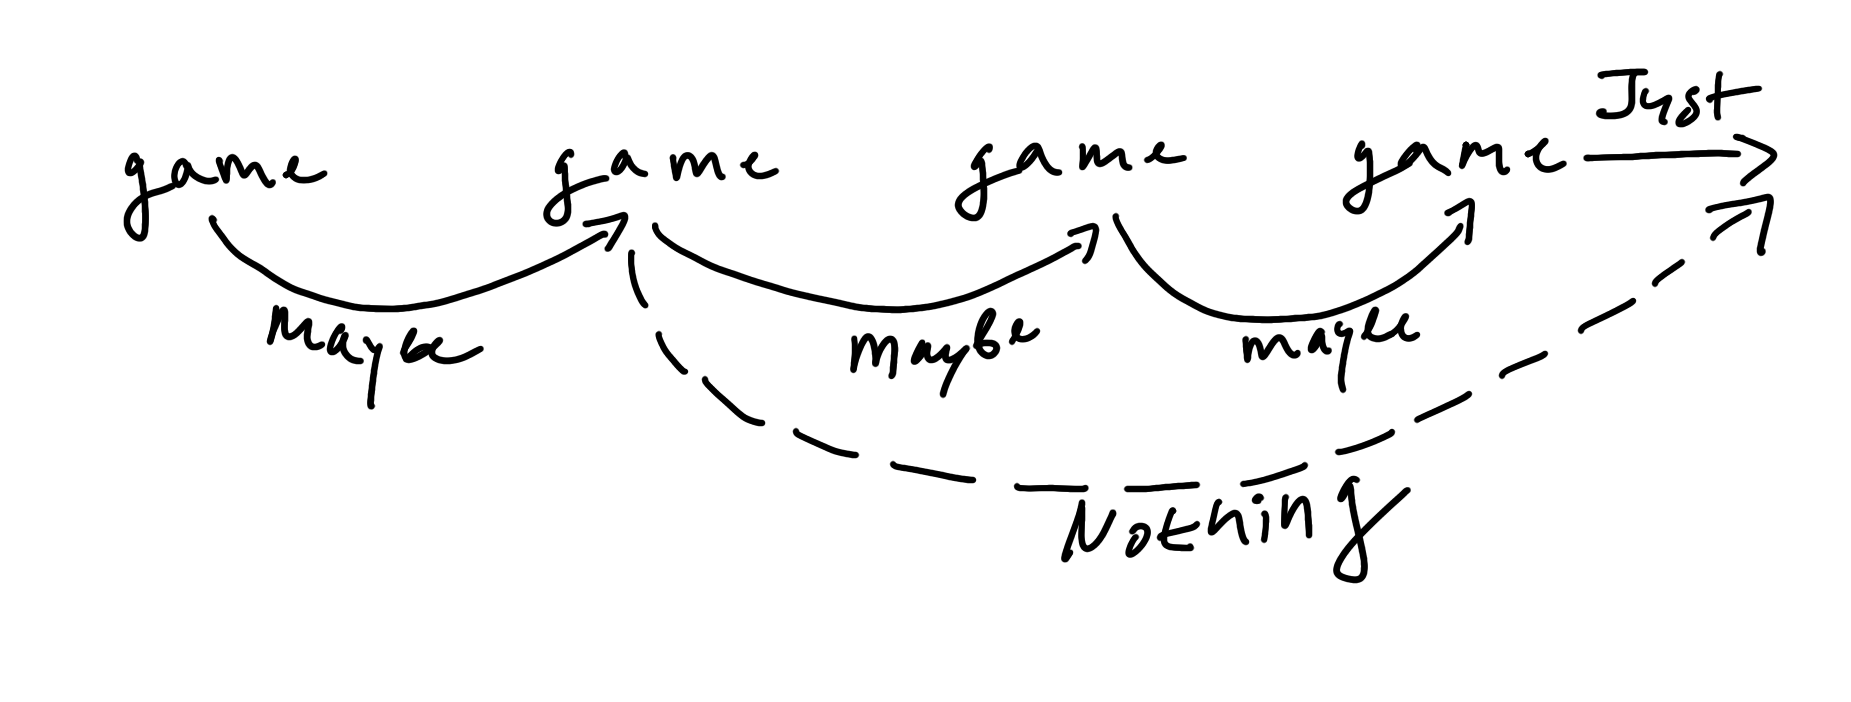
\includegraphics[width=55mm]{images/composition}};
\end{tikzpicture}


\begin{lstlisting}[basicstyle=\small,language=Haskell]
move (Game p w) mv = if dead w (mv p) 
                     then Nothing 
                     else Just $ Game (mv p) w
left g = move g (\(x, y) -> (x-1, y))
...

myWorld = Game {...}

>Just myWorld >>= down >>= down >>= right >>= ...
\end{lstlisting}
\begin{itemize}
  \item Как дефинираме \verb#>>=# за \verb#Maybe#?
\end{itemize}

\begin{lstlisting}[basicstyle=\small,language=Haskell]
Nothing >>= f = Nothing
Just x >>= f = f x
\end{lstlisting}

\end{frame}

\begin{frame}[fragile]
  \frametitle{Какво е IO монада}
\begin{itemize}
  \item Обвързва ``чиста'' стойност с операциите за прочитането ѝ
  \item Позволява композиране на последователни операции, започващи с въведена стойност
  \item Тъй като всяка такава операция зависи от външния свят, резултатът от нея не е чист, макар че изчислението може да е чисто
  \item Това е ролята на \verb#return#: ``опакова'' чиста стойност в контекста на IO
  \item Но МОЖЕМ да изпозлваме чисти изчисления ВЪТРЕ
\end{itemize}
\begin{lstlisting}[basicstyle=\small,language=Haskell]
getLine                                   :: IO(String)
        >>= (\line -> return $ head line) :: IO(Char)
        >>= (\char -> return $ ord char)  :: IO(Int)
\end{lstlisting}
  
\end{frame}

\begin{frame}[fragile]
  \frametitle{do нотация}
\begin{itemize}
  \item Опростява писането при композиране на монадични операции
  \item Подчертва последователността на операциите
  \item Улеснява извличането на чисти стойности
  \item let vs. \verb#<-#
\end{itemize}
\begin{lstlisting}[basicstyle=\small,language=Haskell]
test = do
    line1 <- getLine
    let h1 = head line1
    line2 <- getLine
    let h2 = head line1
    let ascii = max (ord h1) (ord h2)
    return ascii
\end{lstlisting}
\end{frame}


\begin{frame}[fragile]
  \frametitle{IO монада}
\begin{itemize}
  \item Така и така сме в \verb#do#, защо да не изведем нещо?
\end{itemize}
\begin{lstlisting}[basicstyle=\small,language=Haskell]
test = do
    line1 <- getLine
    let h1 = head line1
    putStrLn $ "First letter: " ++ [h1]
    line2 <- getLine
    let h2 = head line2
    putStrLn $ "Second letter: " ++ [h2]
    let ascii = max (ord h1) (ord h2)
    putStrLn $ "Max ascii: " ++ (show ascii)
    return ascii
\end{lstlisting}
\end{frame}


\begin{frame}[fragile]
  \frametitle{Сериализация}
  \begin{tikzpicture}[remember picture,overlay]
    \node[xshift=0,yshift=-14mm,anchor=north] at (current page.north){%
    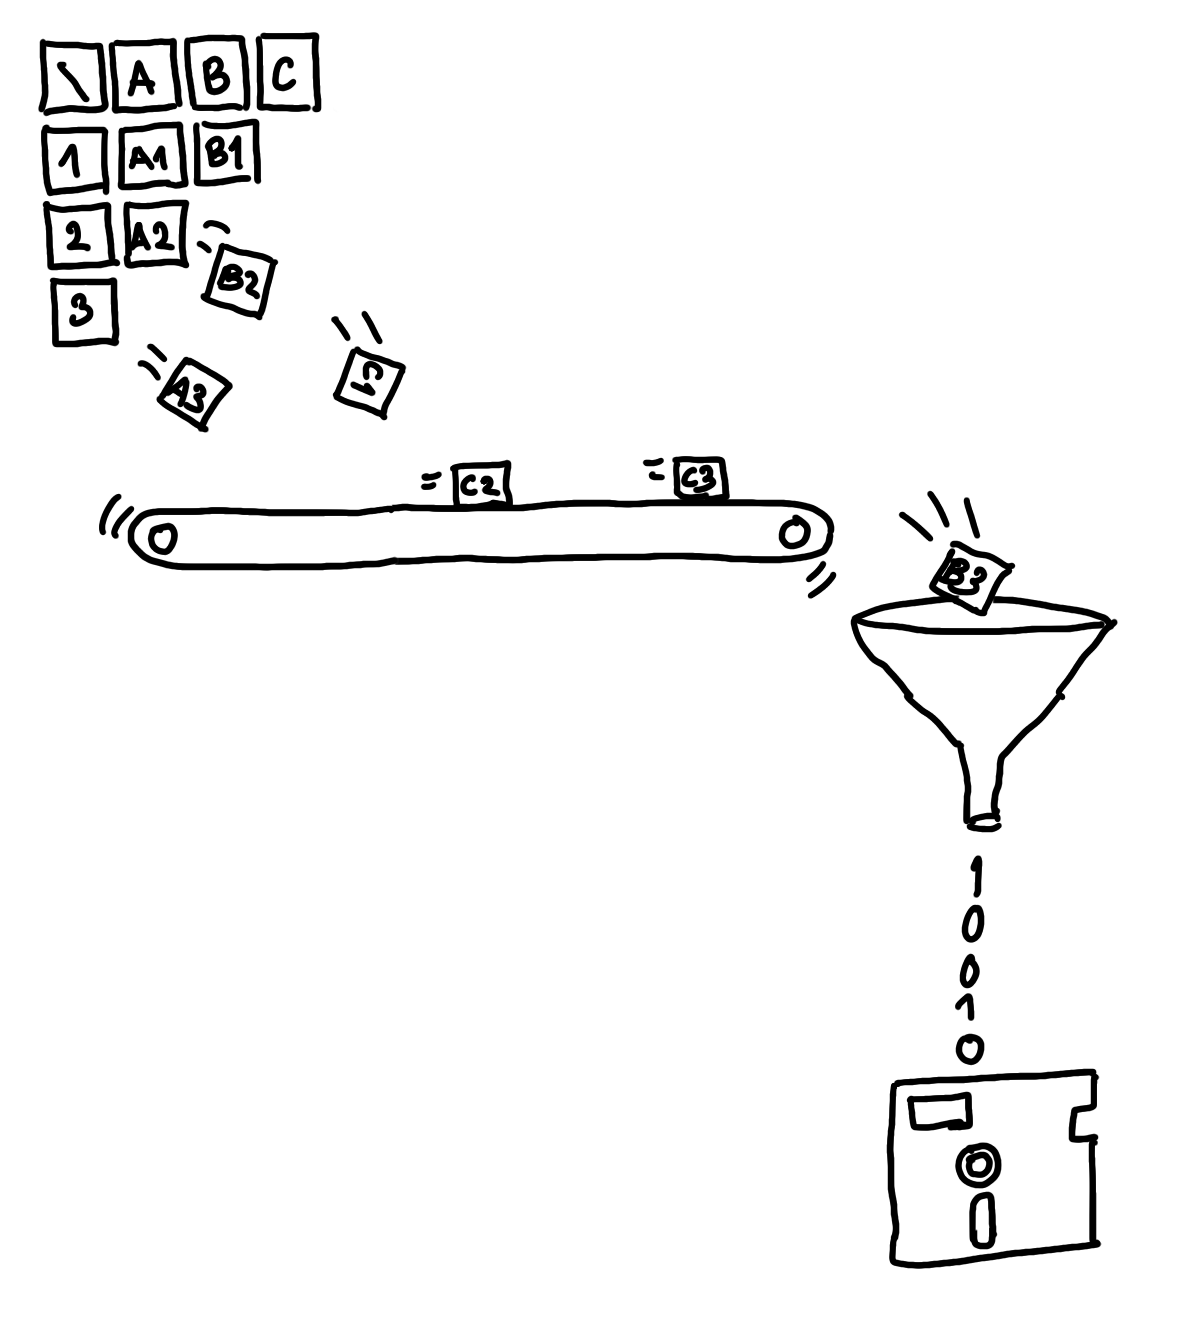
\includegraphics[width=70mm]{images/serialization}};
  \end{tikzpicture}
\end{frame}


\begin{frame}[fragile]
  \frametitle{Сериализация}

\begin{lstlisting}[basicstyle=\small,language=Haskell]
data Gender = M | F
    deriving (Show,Eq)
data Person = Person {name :: String, 
                      gender:: Gender, 
                      birthdate :: (Int,Int,Int)}
    deriving (Show,Eq)
people :: [Person] = 
    [Person {name = "Kalin Georgiev", 
             gender = M, 
             birthdate = (01,01,1981)},
     ...]
\end{lstlisting}

\end{frame}


\begin{frame}[fragile]
  \frametitle{Десериализация}
  \begin{tikzpicture}[remember picture,overlay]
    \node[xshift=0,yshift=-14mm,anchor=north] at (current page.north){%
    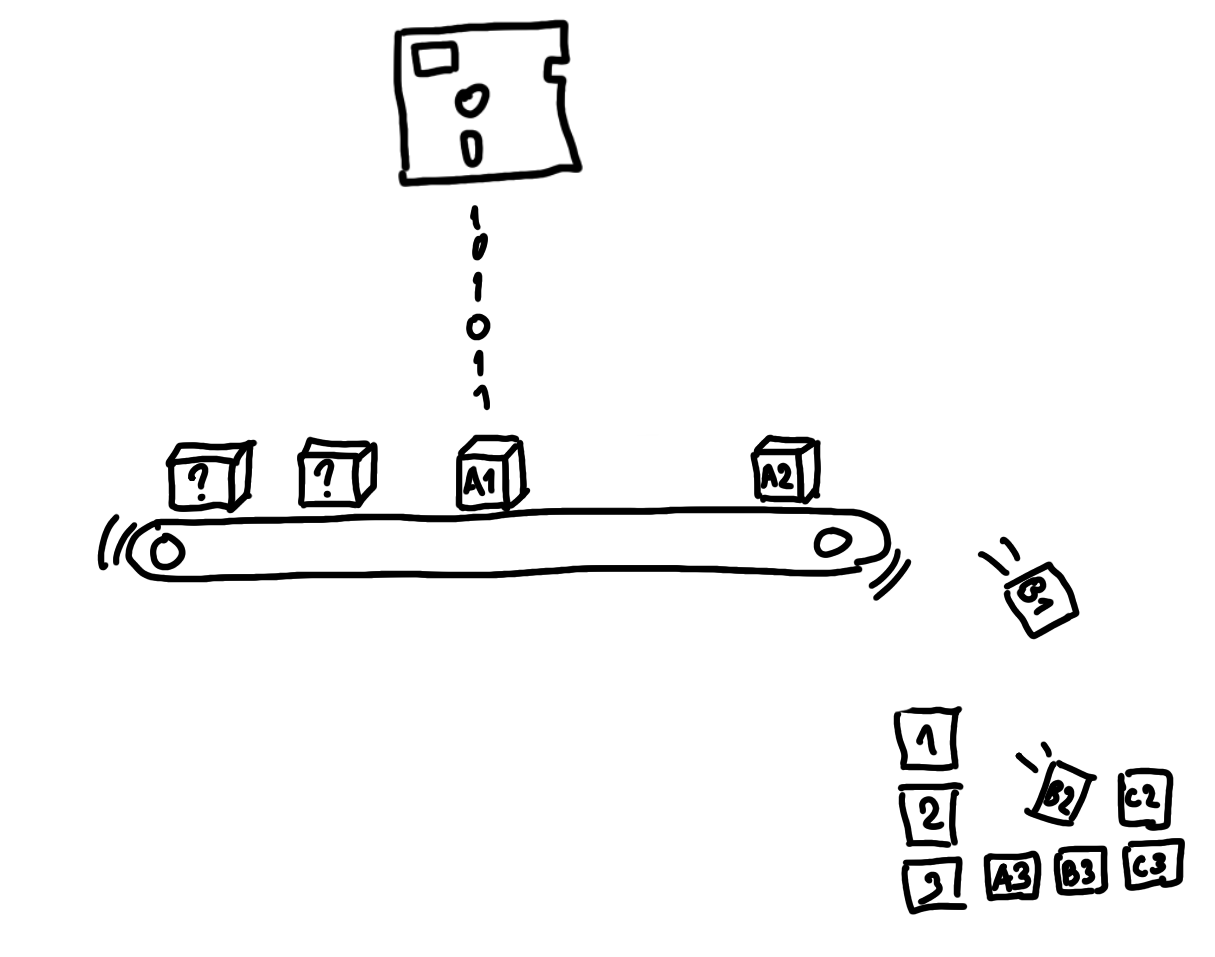
\includegraphics[width=80mm]{images/deserialization}};
  \end{tikzpicture}
\end{frame}



\begin{frame}[fragile]
  \frametitle{Десериализация}

Форматът Comma Seprated Values, \verb#CSV#

\begin{verbatim}
name,gender,birthdate
Kalin Georgiev,M,01-01-1981
Maria Ivanova,F,05-05-2003
\end{verbatim}

\end{frame}


\begin{frame}
  \centerline{Благодаря за вниманието!}
\end{frame}


\end{document}


\begin{columns}[t]
  \begin{column}{0.2\textwidth}

\relscale{0.63}
\begin{lstlisting}
\end{lstlisting}
\relscale{1}

  \end{column}
  \begin{column}{0.8\textwidth}

  \end{column}
\end{columns}


